\documentclass[]{article}
\usepackage{lmodern}
\usepackage{amssymb,amsmath}
\usepackage{ifxetex,ifluatex}
\usepackage{fixltx2e} % provides \textsubscript
\ifnum 0\ifxetex 1\fi\ifluatex 1\fi=0 % if pdftex
  \usepackage[T1]{fontenc}
  \usepackage[utf8]{inputenc}
\else % if luatex or xelatex
  \ifxetex
    \usepackage{mathspec}
  \else
    \usepackage{fontspec}
  \fi
  \defaultfontfeatures{Ligatures=TeX,Scale=MatchLowercase}
\fi
% use upquote if available, for straight quotes in verbatim environments
\IfFileExists{upquote.sty}{\usepackage{upquote}}{}
% use microtype if available
\IfFileExists{microtype.sty}{%
\usepackage{microtype}
\UseMicrotypeSet[protrusion]{basicmath} % disable protrusion for tt fonts
}{}
\usepackage[margin=1in]{geometry}
\usepackage{hyperref}
\hypersetup{unicode=true,
            pdfborder={0 0 0},
            breaklinks=true}
\urlstyle{same}  % don't use monospace font for urls
\usepackage{graphicx,grffile}
\makeatletter
\def\maxwidth{\ifdim\Gin@nat@width>\linewidth\linewidth\else\Gin@nat@width\fi}
\def\maxheight{\ifdim\Gin@nat@height>\textheight\textheight\else\Gin@nat@height\fi}
\makeatother
% Scale images if necessary, so that they will not overflow the page
% margins by default, and it is still possible to overwrite the defaults
% using explicit options in \includegraphics[width, height, ...]{}
\setkeys{Gin}{width=\maxwidth,height=\maxheight,keepaspectratio}
\IfFileExists{parskip.sty}{%
\usepackage{parskip}
}{% else
\setlength{\parindent}{0pt}
\setlength{\parskip}{6pt plus 2pt minus 1pt}
}
\setlength{\emergencystretch}{3em}  % prevent overfull lines
\providecommand{\tightlist}{%
  \setlength{\itemsep}{0pt}\setlength{\parskip}{0pt}}
\setcounter{secnumdepth}{0}
% Redefines (sub)paragraphs to behave more like sections
\ifx\paragraph\undefined\else
\let\oldparagraph\paragraph
\renewcommand{\paragraph}[1]{\oldparagraph{#1}\mbox{}}
\fi
\ifx\subparagraph\undefined\else
\let\oldsubparagraph\subparagraph
\renewcommand{\subparagraph}[1]{\oldsubparagraph{#1}\mbox{}}
\fi

%%% Use protect on footnotes to avoid problems with footnotes in titles
\let\rmarkdownfootnote\footnote%
\def\footnote{\protect\rmarkdownfootnote}

%%% Change title format to be more compact
\usepackage{titling}

% Create subtitle command for use in maketitle
\providecommand{\subtitle}[1]{
  \posttitle{
    \begin{center}\large#1\end{center}
    }
}

\setlength{\droptitle}{-2em}

  \title{}
    \pretitle{\vspace{\droptitle}}
  \posttitle{}
    \author{}
    \preauthor{}\postauthor{}
    \date{}
    \predate{}\postdate{}
  
\usepackage{booktabs}
\usepackage{longtable}
\usepackage{array}
\usepackage{multirow}
\usepackage{wrapfig}
\usepackage{float}
\usepackage{colortbl}
\usepackage{pdflscape}
\usepackage{tabu}
\usepackage{threeparttable}
\usepackage{threeparttablex}
\usepackage[normalem]{ulem}
\usepackage{makecell}
\usepackage{xcolor}

\begin{document}

\hypertarget{migrating-historical-aea-supplements---draft}{%
\section{Migrating historical AEA supplements -
DRAFT}\label{migrating-historical-aea-supplements---draft}}

Since July 16, 2019, the American Economic Association has used the
\textbf{\href{https://www.openicpsr.org/openicpsr/aea}{AEA Data and Code
Repository}} at
\textbf{\href{https://www.openicpsr.org/openicpsr/}{openICPSR}} as the
default archive for its supplements. This archive serves a dual purpose:
to share data with the AEA Data Editor prior to being published, and as
a publication outlet for supplements to articles in AEA journals.

At the time, the AEA also announced that it would migrate the historical
supplements, hitherto stored as ZIP files on the
\href{https://www.aeaweb.org/journals}{AEA website}, into the AEA Data
and Code Repository.

On Oct 1, 2019, openICPSR had 867 deposits, which covered 94 deposits in
the \href{https://www.datalumos.org/datalumos/search/studies}{DataLumos}
archive, 46 in the
\href{https://www.openicpsr.org/openicpsr/search/aerajournals/studies}{AERA
archive}, and 13 in the
\href{https://www.openicpsr.org/openicpsr/search/psid/studies}{PSID}
archive. The \textbf{AEA Data and Code Repository} contained at the time
93 deposits, of which 5 were public, the others awaiting publication of
the associated article.

Between Oct 11 and Oct 13, 2019, the staff at openICPSR ingested 2,552
historical supplements, increasing the size of the openICPSR repository
\textbf{by a factor of 3}, to 3,461. This was only the first part of the
migration, as there are about 1,000 more archives that need to be
migrated.

\hypertarget{increased-findability}{%
\subsection{Increased findability}\label{increased-findability}}

The migrated archives are now available through the
\href{https://www.openicpsr.org/openicpsr/search/aea/studies}{openICPSR
search interface}, the
\href{https://www.icpsr.umich.edu/icpsrweb/ICPSR/search/studies}{general
ICPSR search interface}, as well as through a variety of federated
search interfaces such as
\href{https://toolbox.google.com/datasetsearch/search}{Google Dataset
Search}. For instance, the current AER Editor's supplements can be found
\href{https://www.openicpsr.org/openicpsr/search/aea/studies?start=0\&ARCHIVE=aea\&sort=score\%20desc\%2CTITLE_SORT\%20asc\&rows=25\&q=esther\%20duflo}{here},
\href{https://www.icpsr.umich.edu/icpsrweb/ICPSR/search/studies?start=0\&ARCHIVE=ICPSR\&PUBLISH_STATUS=PUBLISHED\&sort=score\%20desc\%2CTITLE_SORT\%20asc\&rows=50\&q=esther\%20duflo}{here}
and
\href{https://toolbox.google.com/datasetsearch/search?query=esther\%20duflo}{here},
with increasing generality.

\hypertarget{characteristics-of-aea-supplement-data}{%
\subsection{Characteristics of AEA supplement
data}\label{characteristics-of-aea-supplement-data}}

We can describe this subset of the historical supplements in a variety
of ways.

\hypertarget{time-coverage}{%
\subsubsection{Time coverage}\label{time-coverage}}

This is only a subset of all supplements, so what years are covered?

\begin{table}[H]
\centering
\begin{tabular}{r|r}
\hline
year & count\\
\hline
1999 & 2\\
\hline
2000 & 2\\
\hline
2004 & 24\\
\hline
2005 & 280\\
\hline
2006 & 7\\
\hline
2007 & 625\\
\hline
2008 & 1010\\
\hline
2009 & 3918\\
\hline
2010 & 6063\\
\hline
2011 & 6198\\
\hline
2012 & 7394\\
\hline
2013 & 6923\\
\hline
2014 & 11813\\
\hline
2015 & 7511\\
\hline
2016 & 10037\\
\hline
2017 & 11323\\
\hline
2018 & 13574\\
\hline
2019 & 6147\\
\hline
NA & 1865\\
\hline
\end{tabular}
\end{table}

\begin{figure}
\centering
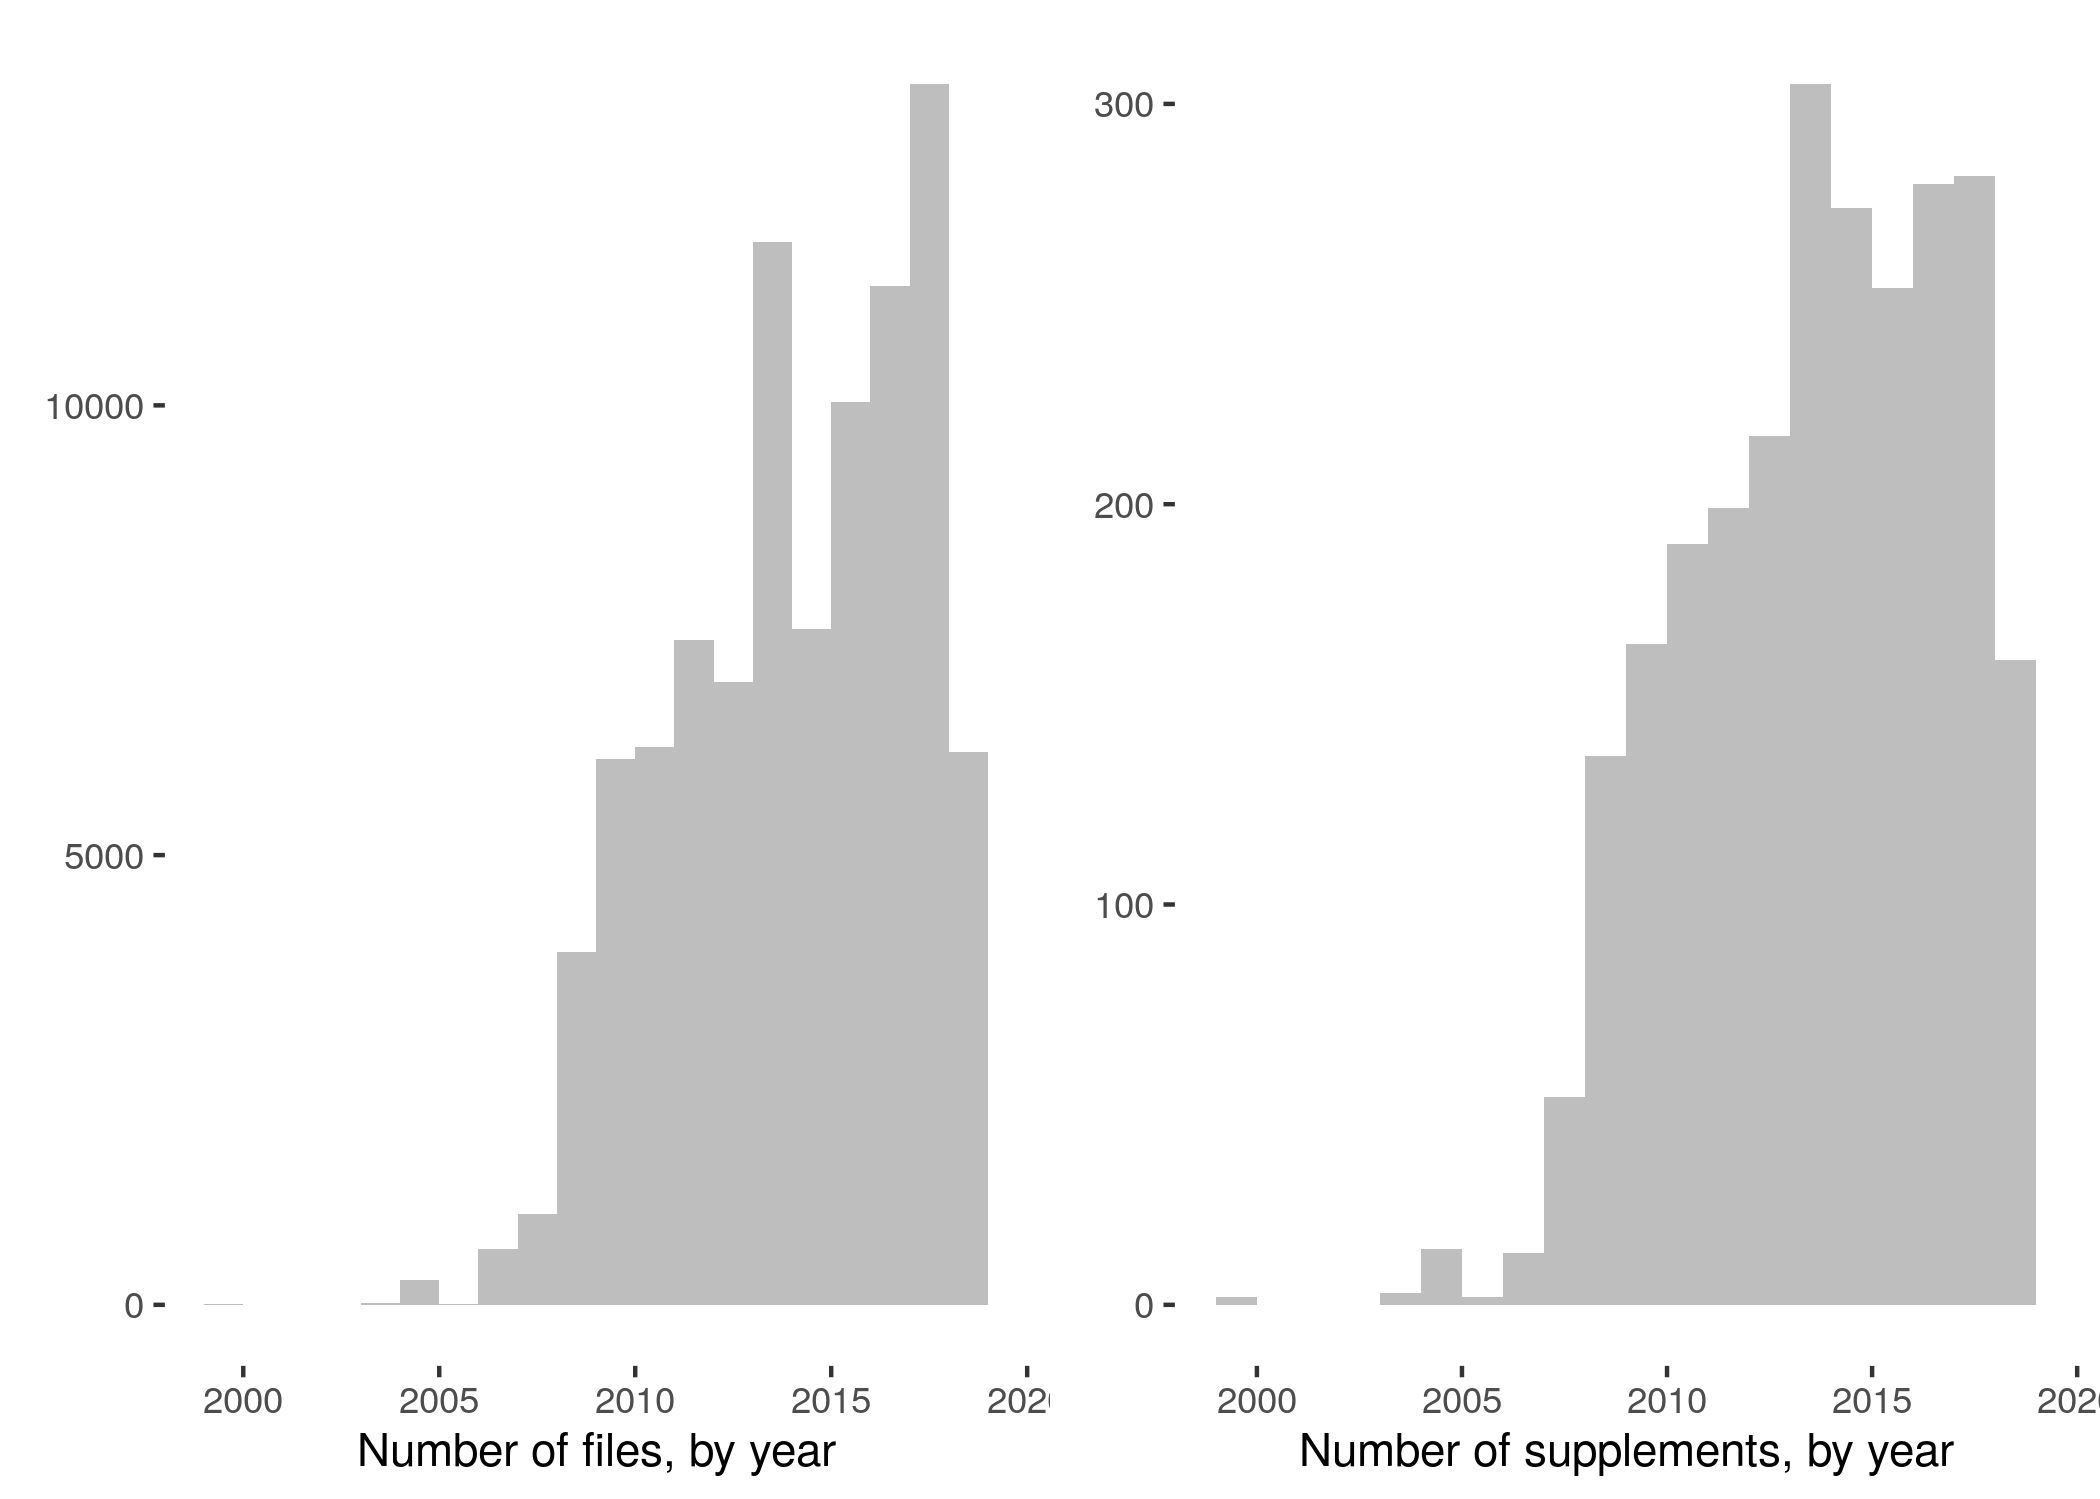
\includegraphics{figure_years.png}
\caption{Distribution across years}
\end{figure}

\hypertarget{number-of-files-per-supplement-and-size-of-supplement}{%
\subsubsection{Number of files per supplement and size of
supplement}\label{number-of-files-per-supplement-and-size-of-supplement}}

\begin{table}[H]
\centering
\begin{tabular}{l|r|r}
\hline
doi & size & count\\
\hline
10.1257/pandp.20181045 & 32782817227 & 795\\
\hline
10.1257/pol.20150168 & 27251086584 & 691\\
\hline
10.1257/app.20170080 & 19924915397 & 236\\
\hline
10.1257/aer.20131496 & 15688843069 & 186\\
\hline
10.1257/app.20160510 & 14419727617 & 465\\
\hline
10.1257/app.6.3.206 & 12190878093 & 45\\
\hline
10.1257/aer.102.2.994 & 10789428265 & 36\\
\hline
10.1257/aer.20121662 & 10334181612 & 622\\
\hline
10.1257/mic.20130164 & 8042445763 & 20\\
\hline
10.1257/aer.20141374 & 6804364827 & 140\\
\hline
\end{tabular}
\end{table}

The 2,552 supplements contain a total of 94,465 files - programs,
documents, datasets. The largest supplement within this group in terms
of file count has 795 files, summing to 30.5 Gb
\href{https://doi.org/10.1257/pandp.20181045}{(Armour, Button, and
Hollands, 2018)}. Note however that among the remaining non-migrated
supplements are very large packages: the largest we have identified has
201,972 files.

\hypertarget{distribution-overall}{%
\subsubsection{Distribution overall}\label{distribution-overall}}

\begin{figure}
\centering
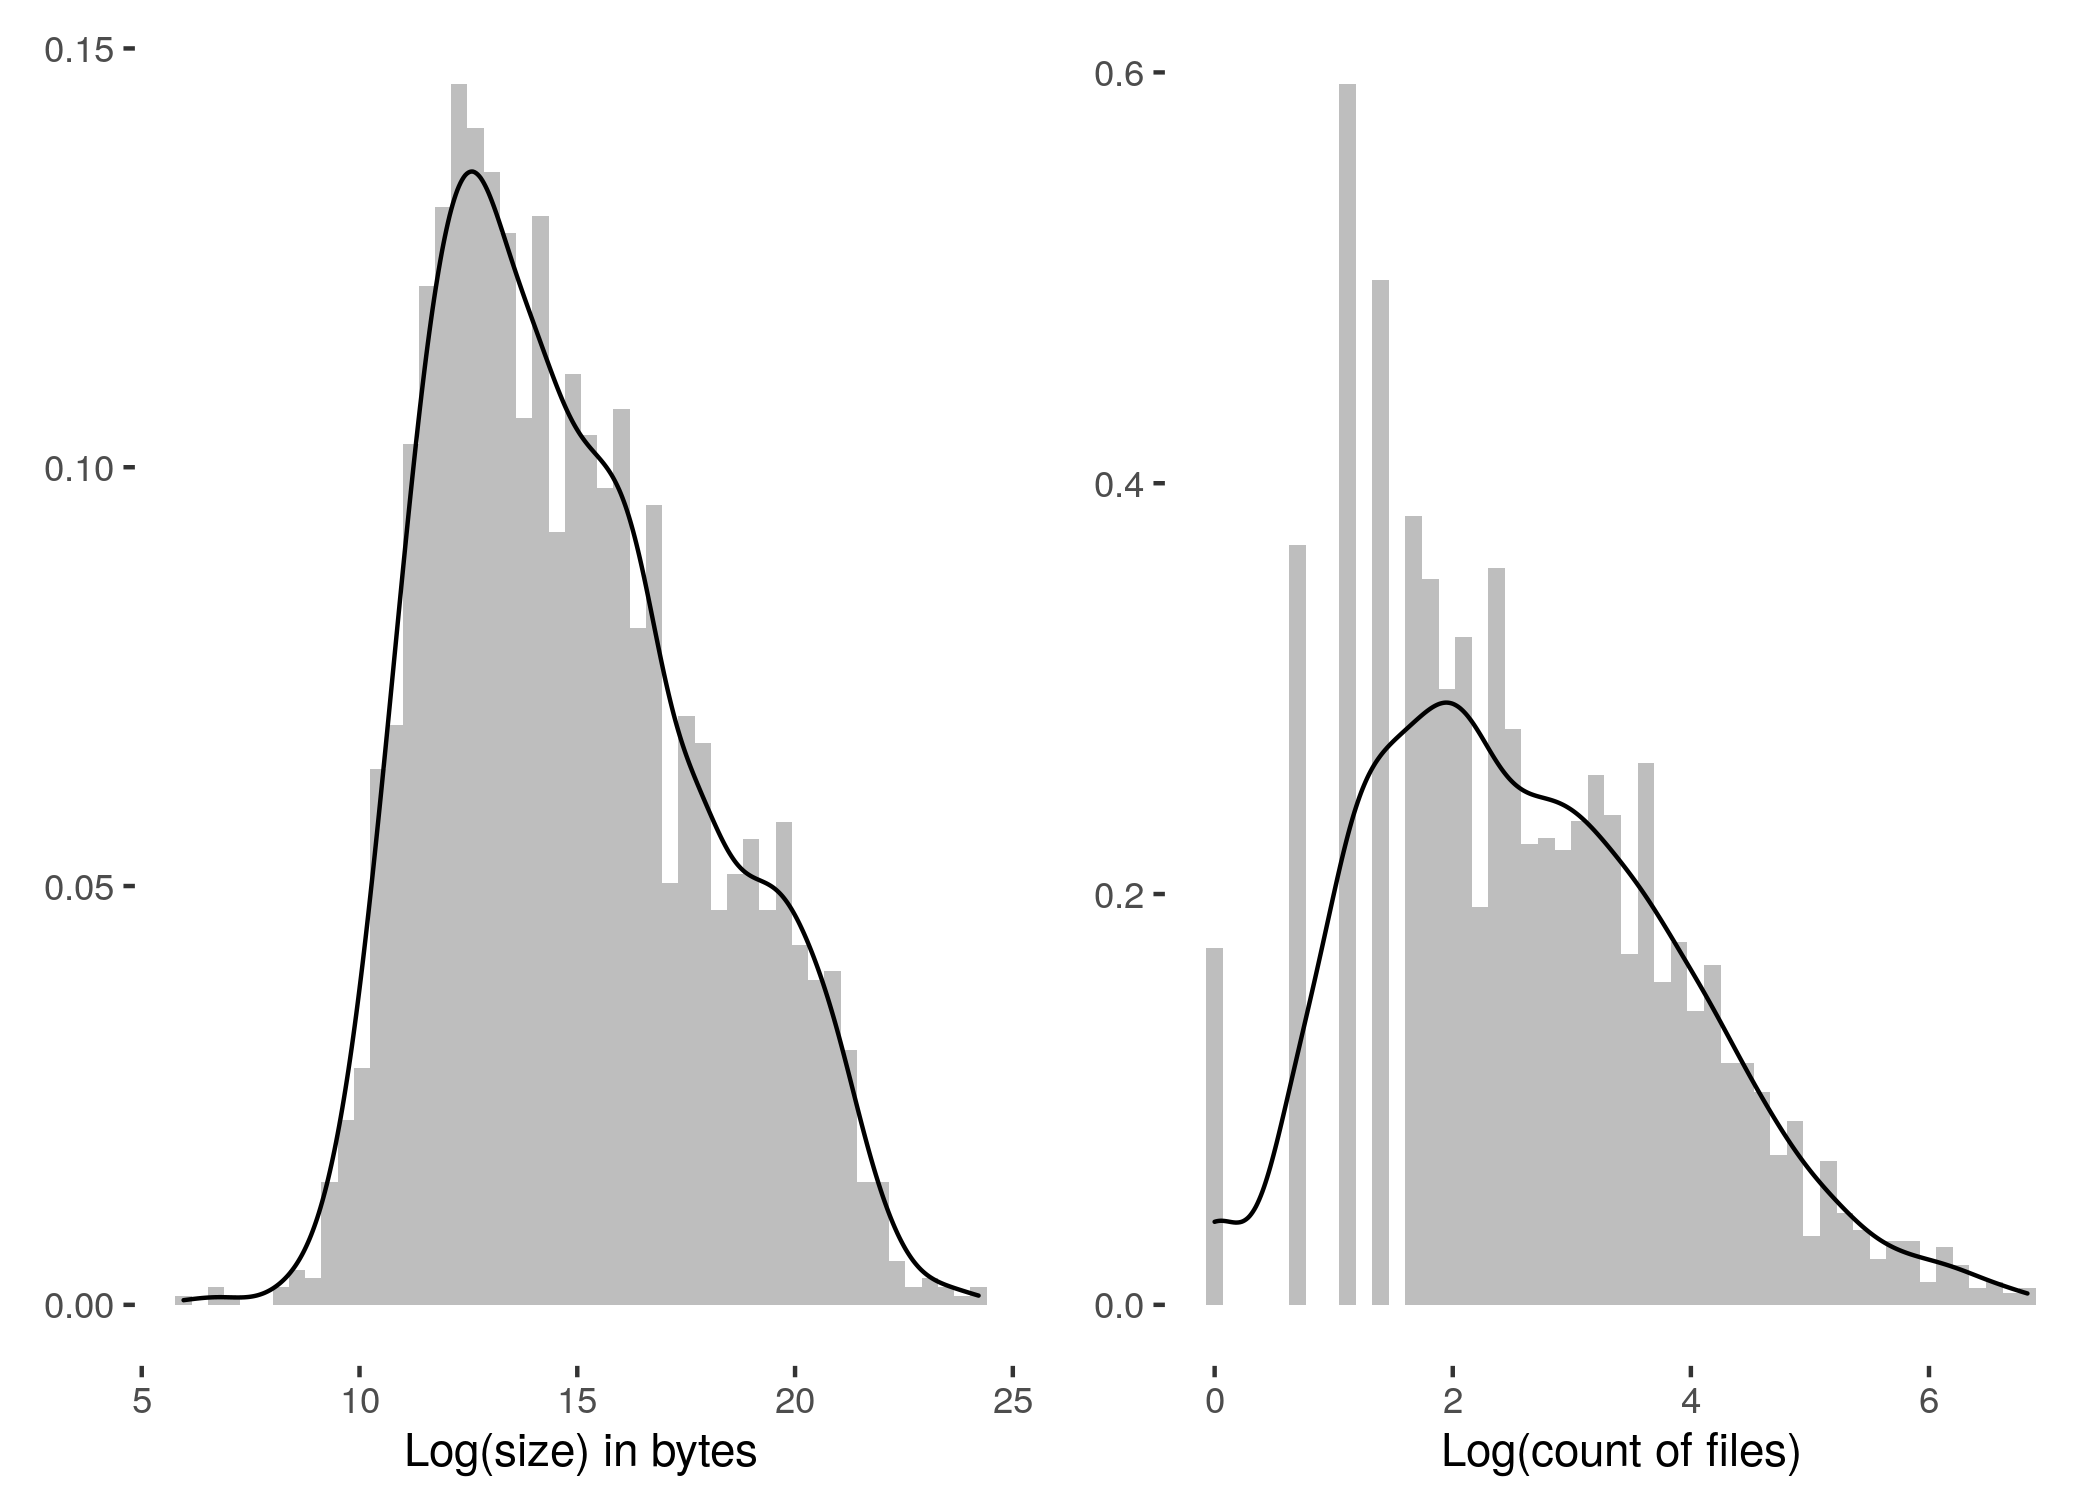
\includegraphics{figure_files.png}
\caption{Distribution of filesizes and filecounts}
\end{figure}

\hypertarget{stats-by-journal}{%
\subsubsection{Stats by journal}\label{stats-by-journal}}

We can look at the size of the supplements globally by journal. The
following table shows cumulative and median size and number of files.

\begin{table}[H]
\centering
\begin{tabular}{l|r|r|r|r|r}
\hline
Journal & Articles & Median Size (Mb) & Cumulative Size (Mb) & Median no. of files & Total no. of files\\
\hline
American Economic Review & 1,238 & 1.4 & 165,552.8 & 13 & 50,310\\
\hline
American Economic Journal: Applied Economics & 363 & 3.1 & 101,969.8 & 10 & 9,979\\
\hline
American Economic Journal: Economic Policy & 351 & 4.2 & 98,574.0 & 12 & 12,585\\
\hline
AEA Papers and Proceedings & 109 & 0.9 & 44,497.3 & 5 & 2,589\\
\hline
American Economic Journal: Macroeconomics & 259 & 1.4 & 14,943.5 & 21 & 10,246\\
\hline
American Economic Journal: Microeconomics & 115 & 1.1 & 12,899.3 & 10 & 5,448\\
\hline
Journal of Economic Perspectives & 115 & 0.8 & 12,755.7 & 7 & 2,833\\
\hline
Journal of Economic Literature & 7 & 17.8 & 432.1 & 67 & 623\\
\hline
American Economic Review: Insights & 3 & 8.2 & 74.7 & 5 & 103\\
\hline
\end{tabular}
\end{table}

\hypertarget{distribution-across-jel-codes}{%
\subsubsection{Distribution across JEL
codes}\label{distribution-across-jel-codes}}

The top 10 JEL codes associated with supplements are:

\begin{table}[H]
\centering
\begin{tabular}{r|r|l|l}
\hline
Number of packages & Pct & JEL & Description\\
\hline
263 & 10.31 & E32 & Business Fluctuations; Cycles\\
\hline
245 & 9.60 & J24 & Human Capital; Skills; Occupational Choice; Labor Productivity\\
\hline
217 & 8.50 & O15 & Economic Development: Human Resources; Human Development; Income Distribution; Migration\\
\hline
214 & 8.39 & D12 & Consumer Economics: Empirical Analysis\\
\hline
207 & 8.11 & J31 & Wage Level and Structure; Wage Differentials\\
\hline
191 & 7.48 & J16 & Economics of Gender; Non-labor Discrimination\\
\hline
183 & 7.17 & J13 & Fertility; Family Planning; Child Care; Children; Youth\\
\hline
176 & 6.90 & I21 & Analysis of Education\\
\hline
162 & 6.35 & D72 & Political Processes: Rent-seeking, Lobbying, Elections, Legislatures, and Voting Behavior\\
\hline
157 & 6.15 & D83 & Search; Learning; Information and Knowledge; Communication; Belief\\
\hline
\multicolumn{4}{l}{\textit{Note: }}\\
\multicolumn{4}{l}{*A supplement can be associated with multiple JEL codes.*}\\
\end{tabular}
\end{table}

\hypertarget{software-used}{%
\subsubsection{Software used}\label{software-used}}

To identify software usage and data formats, we (manually)
\href{../data/original/aea_file_ext.csv}{mapped file extensions} into
known software packages, and classified the file type into a set of
categories:

\begin{table}[H]
\centering
\begin{tabular}{l|r}
\hline
File type & Number of extensions\\
\hline
Program & 66\\
\hline
Document & 36\\
\hline
Data & 26\\
\hline
Junk & 14\\
\hline
Archive & 7\\
\hline
Unknown & 3\\
\hline
Logfile & 2\\
\hline
\end{tabular}
\end{table}

The table below shows the top ten software, by frequency of program
files:

\begin{table}[H]
\centering
\begin{tabular}{r|r|l}
\hline
Number of files & Pct & Software\\
\hline
19676 & 48.37 & Stata\\
\hline
15244 & 37.47 & Matlab\\
\hline
1750 & 4.30 & Fortran\\
\hline
1084 & 2.66 & SAS\\
\hline
659 & 1.62 & R\\
\hline
454 & 1.12 & General\\
\hline
416 & 1.02 & C\\
\hline
291 & 0.72 & Unknown\\
\hline
258 & 0.63 & None\\
\hline
207 & 0.51 & Python\\
\hline
\end{tabular}
\end{table}

The top software with respect to number of files is \textbf{Stata}. Note
that there are 258 supplements that do not contain files that we have
identified as program files (``None'').

More interesting is how many supplements use one or more software:

\begin{table}[H]
\centering
\begin{tabular}{l|r|r}
\hline
Number of Software & N & Percent\\
\hline
1 & 2058 & 80.64\\
\hline
2 & 397 & 15.56\\
\hline
3+ & 105 & 4.11\\
\hline
\end{tabular}
\end{table}

with a maximum of 7 different software packages used in any one of the
supplements. In turn, the number of supplements in which software is
used at least once is reflected in the next table (restricted to at
least 10 mentions):

\begin{table}[H]
\centering
\begin{tabular}{l|r|r}
\hline
Name of Software & Usages & Percent\\
\hline
Stata & 1862 & 72.96\\
\hline
Matlab & 573 & 22.45\\
\hline
None & 258 & 10.11\\
\hline
SAS & 111 & 4.35\\
\hline
R & 97 & 3.80\\
\hline
Fortran & 64 & 2.51\\
\hline
Python & 54 & 2.12\\
\hline
Unknown & 37 & 1.45\\
\hline
C & 34 & 1.33\\
\hline
General & 29 & 1.14\\
\hline
Shell & 29 & 1.14\\
\hline
Windows & 24 & 0.94\\
\hline
\multicolumn{3}{l}{\textit{Note: }}\\
\multicolumn{3}{l}{*Percentage sum to more than 100 percent, since a supplement can use multiple software packages.*}\\
\end{tabular}
\end{table}

\begin{figure}
\centering
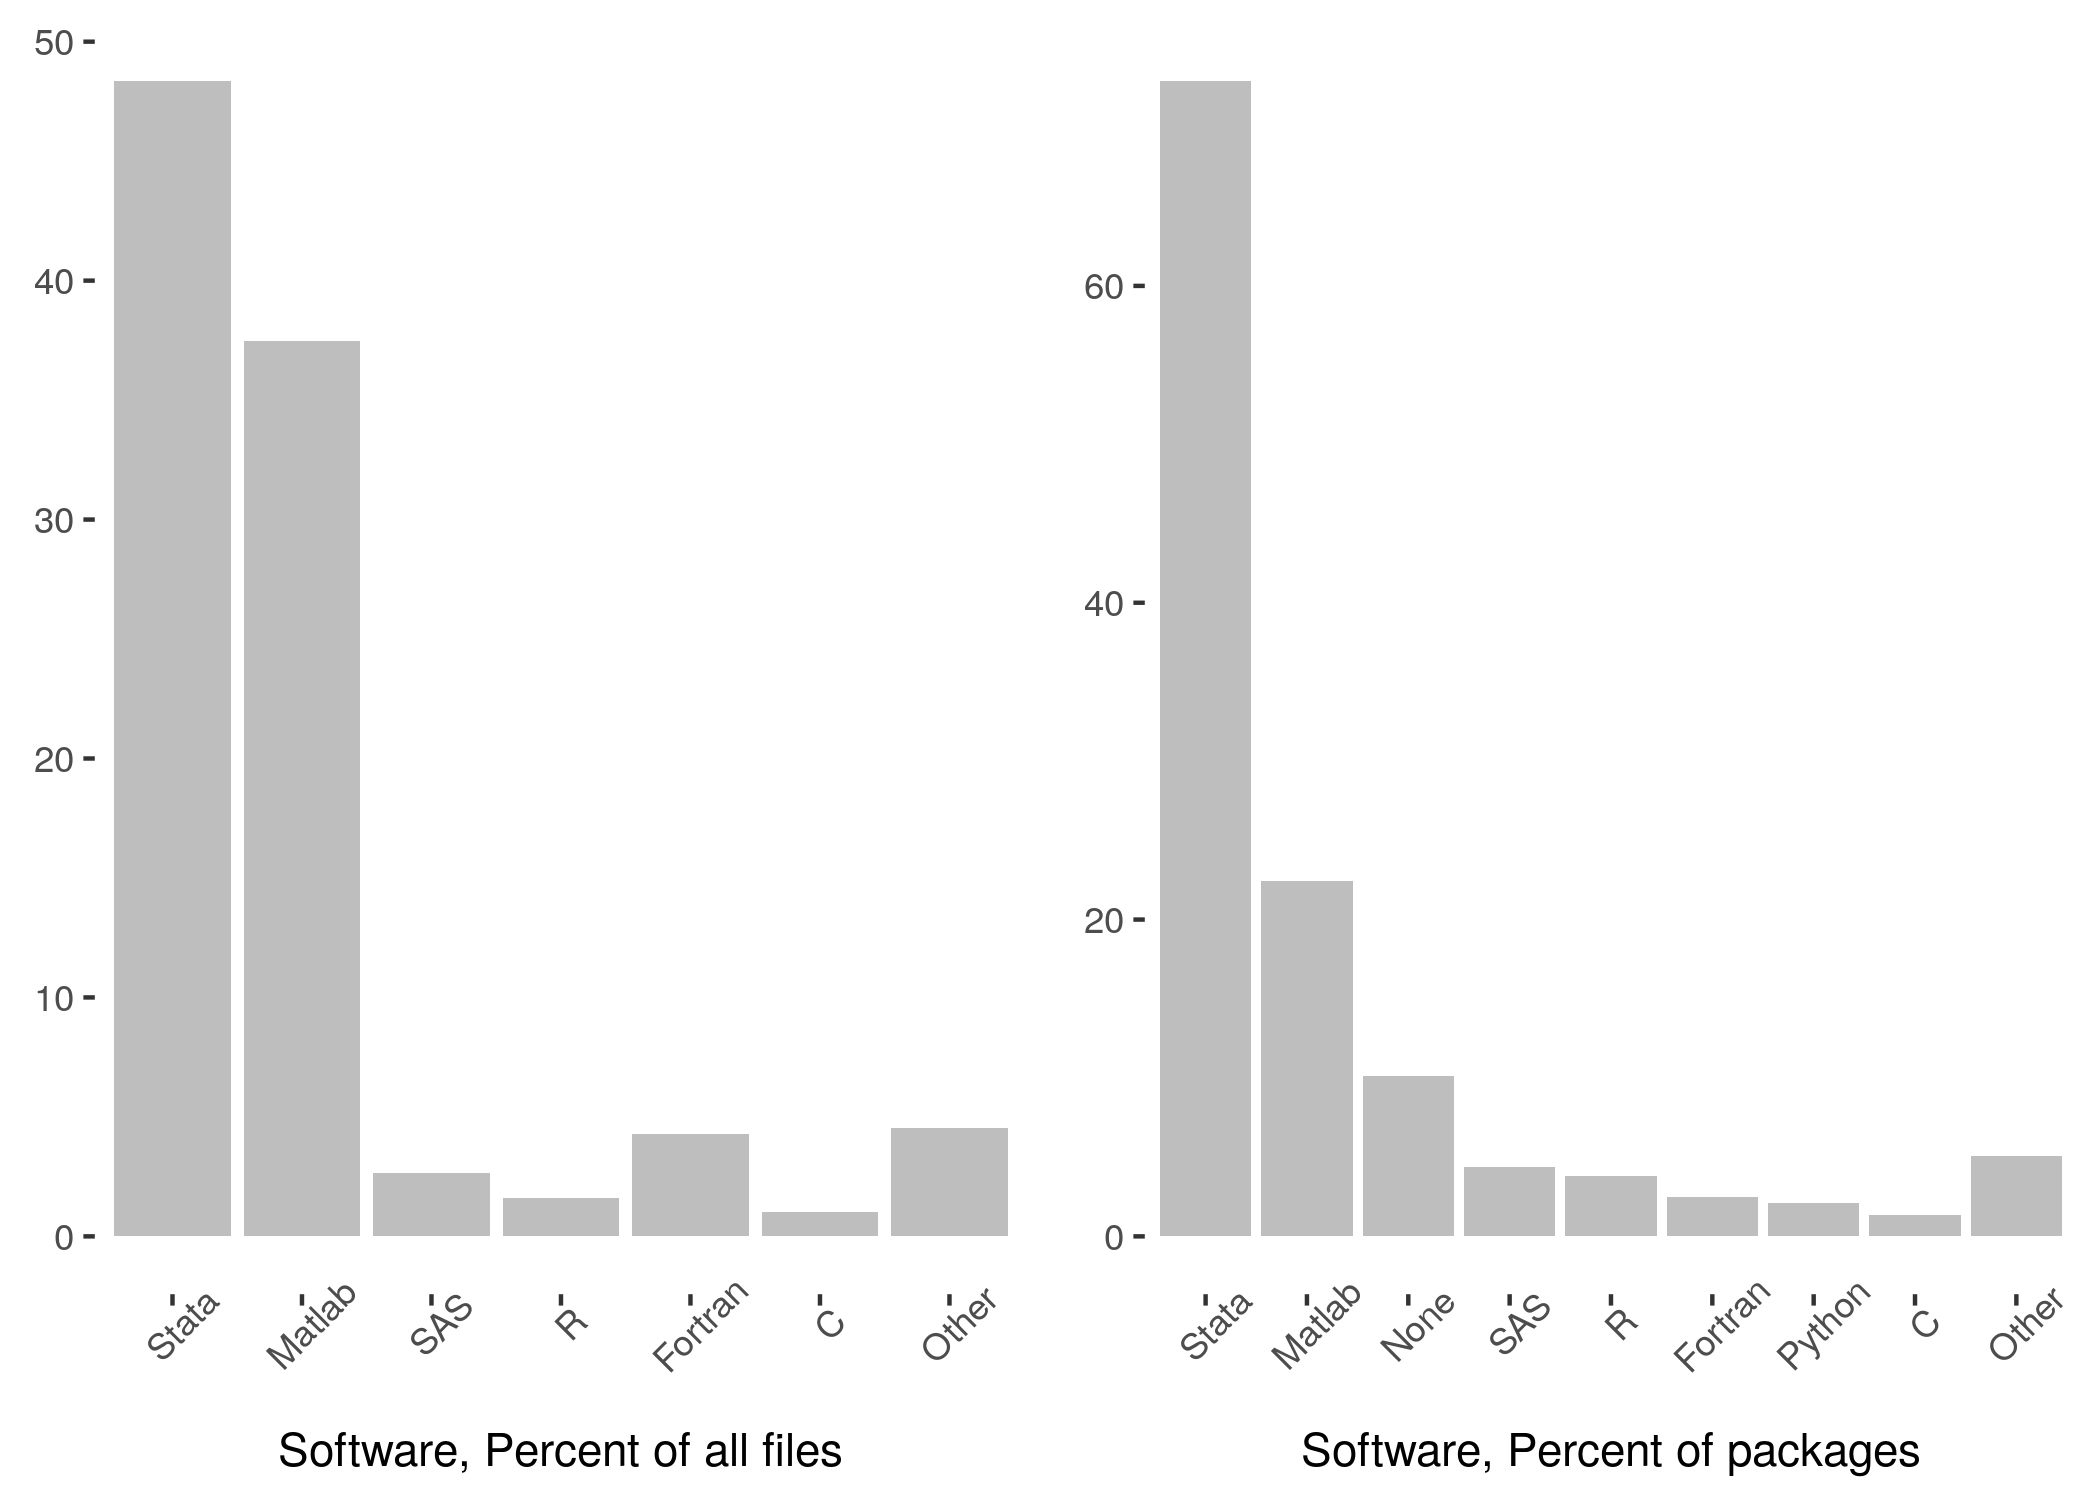
\includegraphics{figure_software.png}
\caption{Distribution of software}
\end{figure}

Clearly, \textbf{Stata} is the most popular statistical software in the
journals of the AEA, followed by \textbf{Matlab}. Note again the 258
supplements that do not contain files that we have identified as program
files (``None'').

\hypertarget{data-formats}{%
\subsubsection{Data formats}\label{data-formats}}

It is somewhat more ambiguous identifying data files, as they come in a
large variety of formats. Furthermore, data might be compressed. In the
following table, we tabulate data files and archives, by the software
package associated with their extension. The data type ``General''
encompasses formats like ``tsv'' or ``csv'' that are not associated with
any particular software, but are nevertheless clearly identifiable as
data files (\href{../data/original/aea_file_ext.csv}{full list
available}). We restrict ourselves to the number of supplements which
contain files with such extensions.

\begin{table}[H]
\centering
\begin{tabular}{l|r|r}
\hline
Name of Software & Usages & Percent\\
\hline
Stata & 1392 & 44.90\\
\hline
Excel & 682 & 22.00\\
\hline
General & 547 & 17.65\\
\hline
Matlab & 242 & 7.81\\
\hline
Archive & 179 & 5.77\\
\hline
SAS & 38 & 1.23\\
\hline
R & 9 & 0.29\\
\hline
OpenOffice & 5 & 0.16\\
\hline
Unknown & 3 & 0.10\\
\hline
SPSS & 2 & 0.06\\
\hline
Julia & 1 & 0.03\\
\hline
\multicolumn{3}{l}{\textit{Note: }}\\
\multicolumn{3}{l}{*Percentage sum to more than 100 percent, since a supplement can use multiple software packages.*}\\
\end{tabular}
\end{table}

\hypertarget{metadata}{%
\subsection{Metadata}\label{metadata}}

When planning the migration, the preservation of existing metadata - the
information about the data and code - was important. The AEA Data Editor
worked with the openICPSR staff to enhance the data infrastructure,
adding the capability to store and display JEL codes in addition to
subject terms. Going forward, in addition to adding the JEL codes that
also describe the linked article, authors can add metadata such as
\emph{geographic coverage}, \emph{funding sources}, \emph{time periods},
\emph{geographic units} as well as \emph{units of observation}, greatly
enhancing the ability of researchers to find data through the openICPSR
search interface.

Two important caveats apply, however. First, none of the additional
metadata exists for the historical archives. Second, the openICPSR
search interface only allows to search for these in an implicit way,
i.e., one can search for ``J31'' because it is unlikely to appear as
anything else, but there is no selection by specific JEL codes currently
possible. The ability to do so is planned for a later implementation.

\hypertarget{references}{%
\subsection*{References}\label{references}}
\addcontentsline{toc}{subsection}{References}

\hypertarget{refs}{}
\leavevmode\hypertarget{ref-Armour_2018}{}%
Armour, Phillip, Patrick Button, and Simon Hollands. 2018. ``Disability
Saliency and Discrimination in Hiring.'' \emph{AEA Papers and
Proceedings} 108. American Economic Association: 262--66.
\url{https://doi.org/10.1257/pandp.20181045}.


\end{document}
